\chapter{系统实现}
\thispagestyle{fancy}
本章介绍系统的实现细节,包括数据获取,数据分析和数据呈现。

\section{数据获取}
\subsection{爬取微博数据}
新浪微博每天会产生一亿多条微博\cite{CN12},我们不可能爬取所有的微博数据,因此需要设计一个爬虫可以高效地抽取一个样本数据。我们使用了 Haixin Ma 等人\cite{haixin13}开发的爬虫从新浪微博抓取数据。爬虫使用 Sina Weibo API 抓取用户档案,社交关系和微博。抓取的过程如图 4-1 所示。
\begin{figure}[!h]
\centering
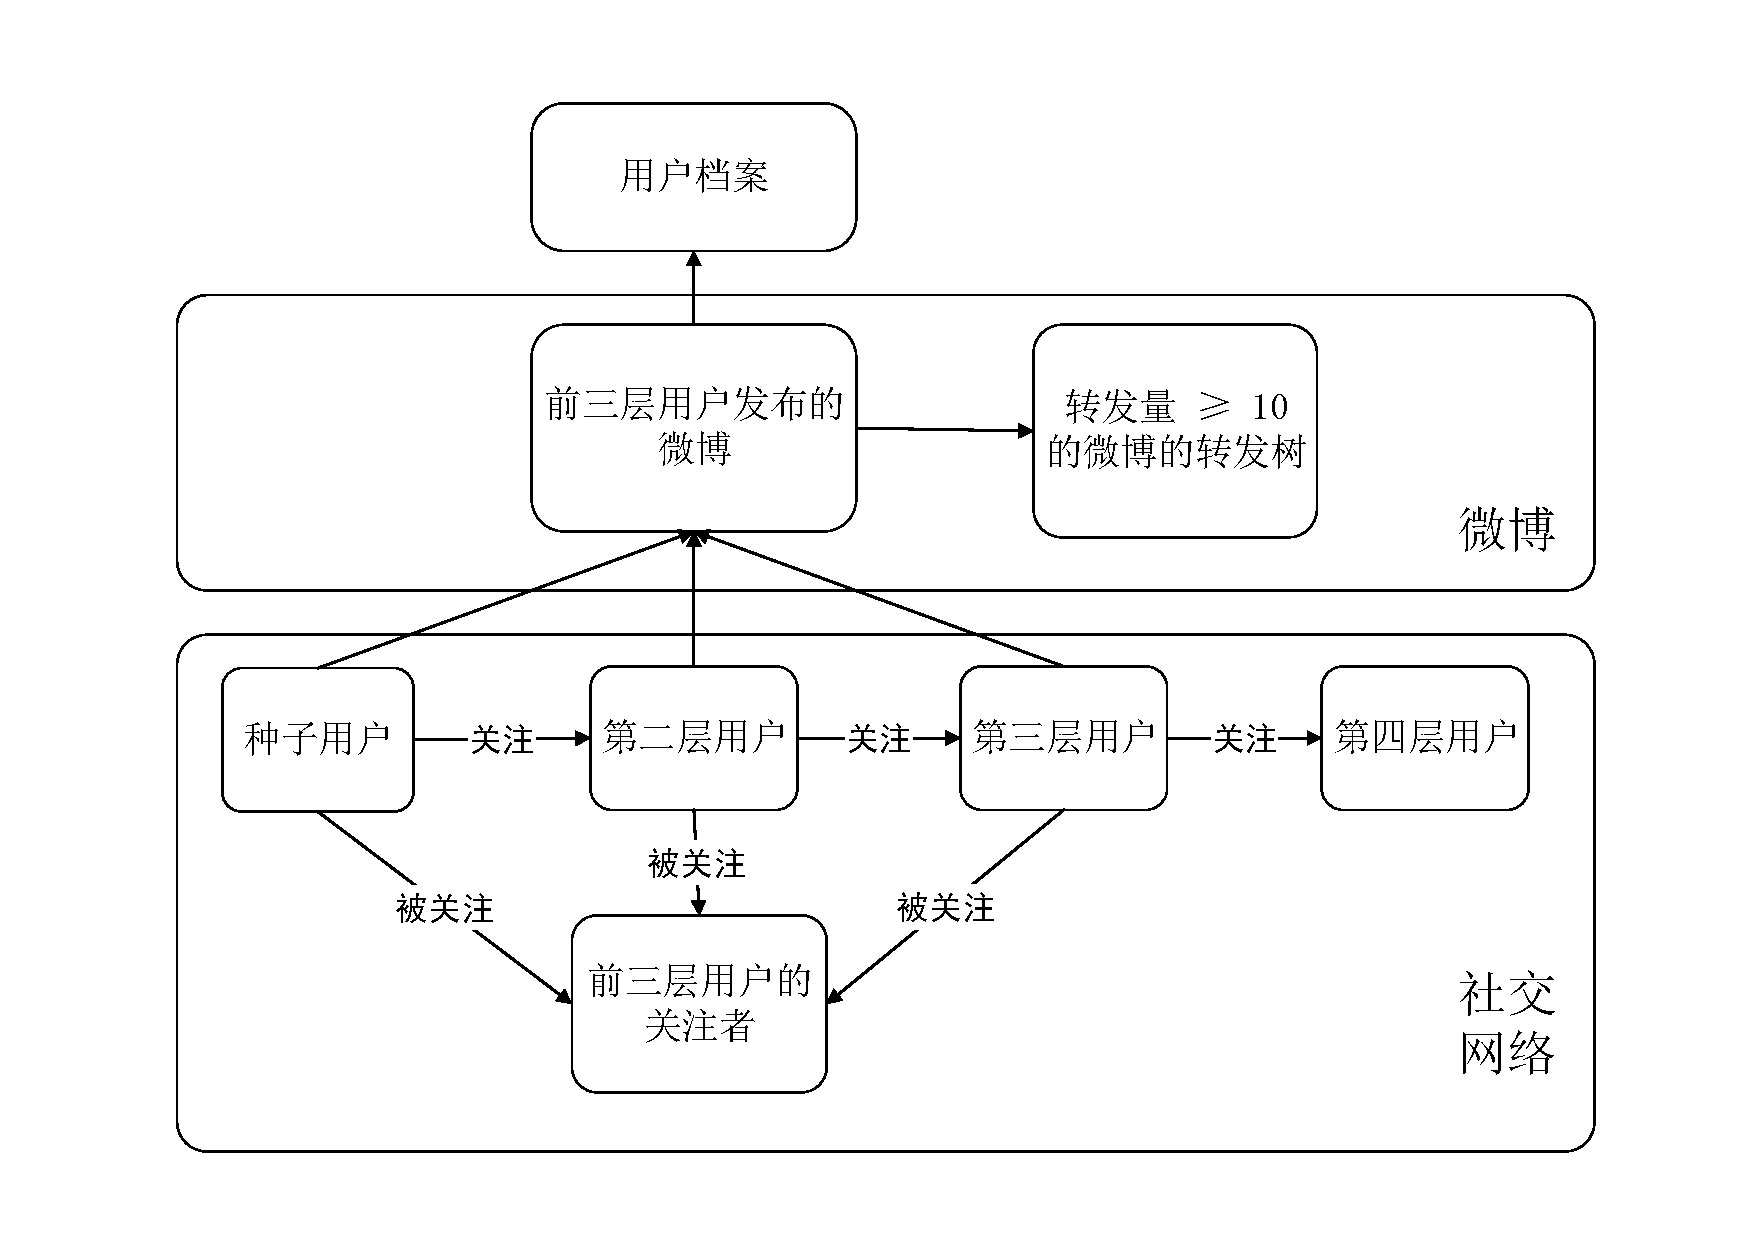
\includegraphics[width=\textwidth]{crawler}
图 4-1 数据抓取
\caption{crawling data}
\end{figure}

爬虫从 32 个种子用户出发,以广度优先的方式通过关注关系寻找下层用户,收集了前三层用户的微博,及转发量大于 10 的微博的转发树。

\subsection{爬取维基百科页面}
维基百科提供了 MediaWiki API 支持应用程序爬取维基百科页面,我们使用 HTTP POST\cite{http} 动作,以话题名为参数,爬取话题在维基百科上的介绍页面,返回的数据为 HTML 格式。

\section{数据分析}
\subsection{MapReduce 计算}
我们抓取的微博数据以 JSON (JavaScript Object Notation)\cite{json} 格式储存,(这里为了方便展示,我们将微博的各属性分行显示,实际上一行数据含有多条这样的微博,此外这里隐去了无关的部分)。

\lstset{emph={created_at, text, user, province, city, reposts_count, comments_count}, emphstyle=\textbf}
\lstinputlisting[frame=single]{status.js}

created\_at 表示微博发布的时间; text 表示微博的正文;user 表示微博用户的信息;其中包括用户的位置信息:province(省) 和 city(市);reposts\_count 和 comments\_count 表示微博的转发量和评论量。在解析过程中,我们将其以字符串的形式读入,然后反序列化为一个 JSON 对象,这样我们可以调用 JSON 对象暴露的方法获取上述属性值。

我们为每一话题定义了对应的正则表达式。如果一条微博中含有能匹配某个正则表达式的字符串,则表示它出现了该话题。如一个话题是 “谷歌退出中国”,对应的正则表达式为 “(Goolge|google|谷歌).*退出.*中国”,则一条含有 “Google 正式退出了中国” 的微博中就出现了 “谷歌退出中国” 这一话题。

我们应用 MapReduce 计算框架在时间,地域,情绪等维度上对数据进行分组和聚合。首先我们通过伪代码解释 Map 和 Reduce 的过程。regexToTopicMap 是一个从正则表达式映射到话题的哈希表。

\begin{algorithm}
\caption{map(key, value, context)}
\label{alg1}
\begin{algorithmic}[1]
\STATE $tweetList \leftarrow value.deserialize()$
\FORALL {$tweet$ in $tweetList$}
\STATE $text \leftarrow tweet.getText()$
\STATE $count \leftarrow tweet.getCount()$
\FORALL {$regex$ in $regexToTopicMap$}
\IF {$tweet$ matches $regex$}
\STATE $topic \leftarrow regexToTopicMap.get(regex)$
\STATE $context.write(topic, count)$
\ENDIF
\ENDFOR
\ENDFOR
\end{algorithmic}	
\end{algorithm}

在 Map 阶段,我们根据话题对微博进行分组。Map 阶段的输入以行为单位,key 是该行在文件中的偏移量,value 是该行的数据,在这里是包含多条微博的字符串。我们将所有这样的字符串反序列化成 JSON 对象。之后,我们从中获取 text (微博正文)和 count (统计量,如 reposts\_count,comments\_count 等)。下面我们遍历 regexToTopicMap 的所有键,寻找能够匹配 text 的正则表达式。如果匹配成功,则输出话题和统计量的键值对。MapReduce 框架会自动根据话题对 Map 输出进行分组,作为 Reduce 的输入。

在 Reduce 阶段,我们对各组话题的统计数据进行聚合。Reduce 阶段的输入以话题为单位,key 是某一话题,valueList 是出现了这一话题的所有微博的统计量列表。在这个例子中,我们将统计量相加进行求和操作,当然,我们也可以求得最大值,平均值等其他统计结果。

\begin{algorithm}
\caption{reduce(key, valueList, context)}
\label{alg2}
\begin{algorithmic}[1]
\STATE $sum \leftarrow 0$
\FORALL {$value$ in $valueList$}
\STATE $sum \leftarrow sum + value$
\ENDFOR
\STATE $context.write(key, sum)$
\end{algorithmic}
\end{algorithm}

下面我们具体解释对 MapReduce 框架的应用过程。根据功能设计,我们需要统计话题的讨论数。由于 Reduce 阶段输入的 valueList 对应一个话题,其中的 一个 value 表示话题出现了一次,那么它的长度就是话题的讨论数。在对不同维度进行聚合操作时,我们只需要修改 Map 输出的键值。在分析话题讨论数随时间的变化趋势时,我们取出 created\_at 字段,将它和话题拼接在一起作为 Map 输出的键(用'\textbackslash t'隔开)。而在分析地域分布时,则是取出 province 字段,统计一个话题在一个省的讨论数。源数据的 province 是一个编号,新浪微博提供了编号和省份名的映射表,包括各省,直辖市,港澳台,海外和其它。为了地图显示方便,我们忽略海外和其它的数据。对于和情绪词有关的统计,我们需要增加一个循环,遍历情绪词表,寻找微博正文中的完全匹配。我们将话题,情绪词和情绪特征的拼接词作为 Map 输出的键。 

\subsection{抽取话题简介}
在数据获取模块,我们从维基百科爬取了话题的 HTML 页面,但话题的内容不是展示的重点,我们只需要抽取话题简介。维基百科通常会在第一段正文给出一个词条的简介。如图 4-2 的红框部分。

\begin{figure}[t]
\centering
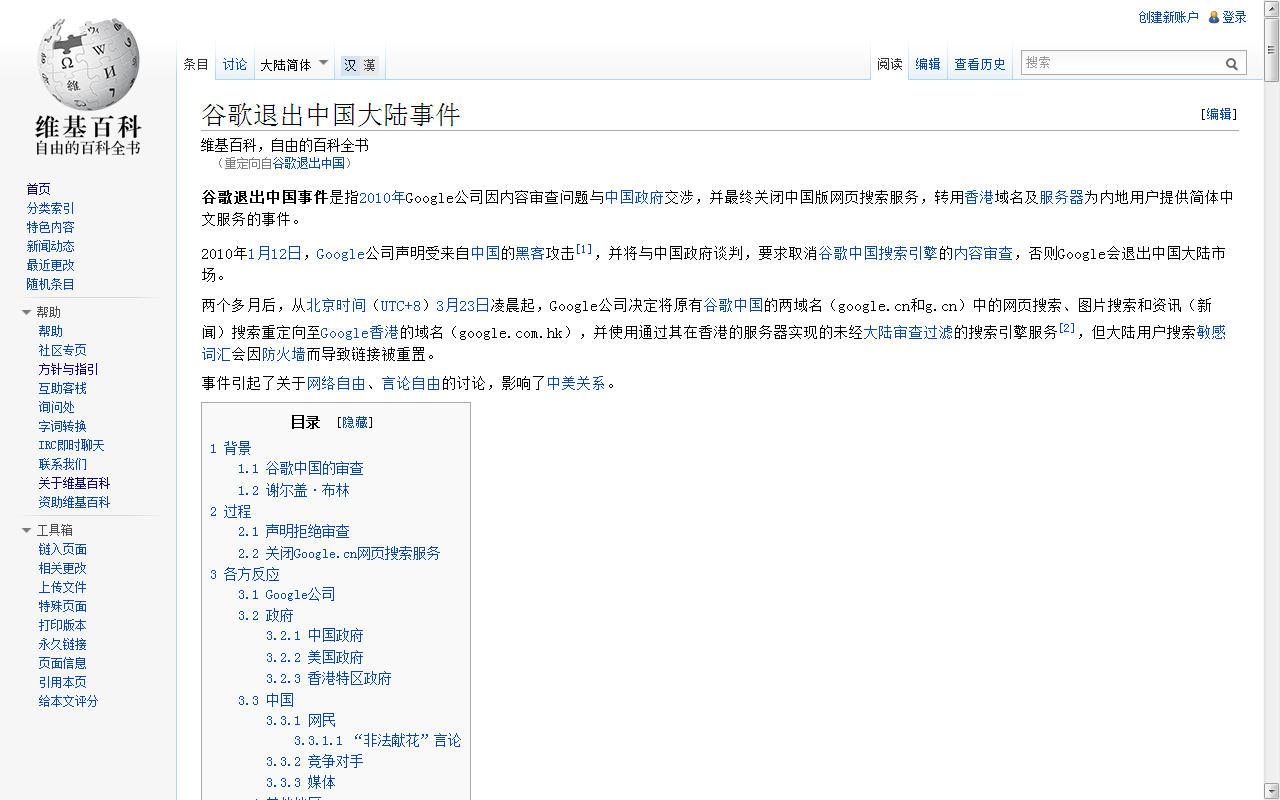
\includegraphics[width=\textwidth, height=0.4\textheight]{wikipedia}
图 4-2 维基百科
\caption{wikipedia}
\end{figure}

这对应到 HTML,就是第一组 “<p>" 和 “</p>” 包含的内容,我们将这段内容取出,去除其中的 HTML 标签(如 “<b></b>” 等),就生成了话题的简介。


\subsection{数据存储}
Google App Engine 的 Datastore 数据存储区提供了批量上传导入数据(CSV 或者 XML 文件)的功能。数据存储区是非关系型的,它的存储单位是实体 (Entity),表 4-1 是 Datastore 与 关系型数据库(RDBMS)类似概念的比较。
\begin{table}[!h]
\centering
表 4-1 Datastore 与 RDBMS 的比较 
\caption{Datastore vs. RDBMS} 
\vspace{\baselineskip}
\begin{tabular}{cc}
\toprule[1.5pt]
\head{Datastore} & \head{RDBMS} \\
\midrule
Kind & Table \\
Entity & Row \\
Property & Column \\
Entity key & Primary key \\
\bottomrule[1.5pt]
\end{tabular}
\end{table}

在上传数据之前,需要先在配置文件中定义一个实体的种类(Kind)和属性(Property)。例如我们要上传话题的讨论数,评论量和转发量,可以定义一个 topic\_count 种类,实体的属性包括 topic (话题),tweets\_count (讨论数),comments\_count (评论数)和 repost\_count (转发数)。Google App Engine 提供了在网页端查询数据的服务,图 4-3 即是数据存储区中的数据格式,它还包括存储区自动生成的 Entity key,作为实体的唯一标识。

\begin{figure}[!h]
\centering
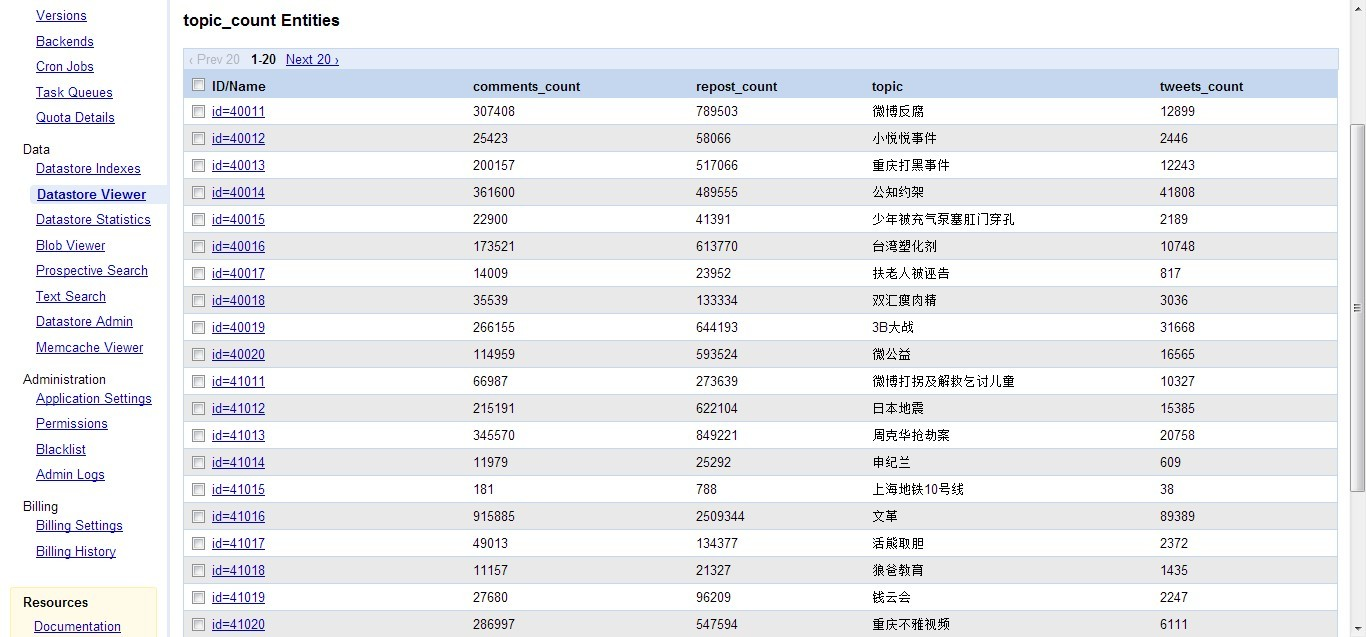
\includegraphics[width=\textwidth]{gae}
图 4-3 GAE 数据存储
\caption{GAE Datastore Entity}
\end{figure}

\section{数据呈现}
我们构建了一个基于 Google App Engine 的 Java Web 应用。在客户端,我们借助 jQuery 操纵 HTML 文档,实现动画效果,监听事件,因此只需要一个页面即能呈现各组数据,而不需要跳转。另外,我们直接调用 jQuery 的 Ajax 方法完成客户端和服务器端的数据传输。

\begin{figure}[!h]
\centering
\includegraphics[width=\textwidth, height=0.4\textheight]{jQuery}
图 4-4 网页交互
\caption{interaction}
\end{figure}

如图 4-4 所示,当我们点击页面触发事件时,jQuery 的 Ajax 方法从客户端发起一个 XmlHttpRequest 请求,在服务器端由相应的 Java Servlet\cite{servlet} 处理请求(如从 High Replication 存储区读取某个话题的微博数),返回序列化后的结果(如 JSON 字符串),触发 jQuery 重新绘制页面。

我们使用了基于 JavaScript 的可视化工具 Google Chart Tools 和 Data-Driven Documents (D3)。

在绘制折线图,柱状图和地域图时,我们加载 Google Chart Tools 的 corechart 包(包括 linechart,columnchart,geochart),使用 DataTable\footnote{ https://developers.google.com/chart/interactive/docs/reference} 对象将返回的 JSON (嵌套)结构转化为图表(行列)结构。

在绘制情绪词云图时,我们调用了基于 D3 的 d3-cloud\footnote{https://github.com/jasondavies/d3-cloud} JavaScript 词汇云图实现。情绪词云图的基本思路是根据情绪词的出现次数决定其在云图中显示字体的大小,这样用户一眼就能辨识出话题中的主要情绪。我们设计了一个简单而显示效果不错的函数(4.1)来实现这一点,其中 size 是字体大小,count 是情绪词出现次数,max 是所有 count 的最大值。
\begin{equation}
 size = count / max * 90 + 10
\end{equation}
同时,我们将相同情绪特征的情绪词用同一种颜色表示,并且和柱状图中对应情绪特征的颜色一致。这样用户可以很方便地通过情绪特征找到它下面的情绪词,更细粒度地了解话题中的情绪。



